% 大学物理实验报告

\documentclass[UTF8]{ctexart}

\usepackage{amsmath}        %数学公式
\usepackage{cases}          %联立编号
\usepackage{cite}           %引用
% \usepackage{enumitem}       %编号

\usepackage{graphicx}       %插入图片
\usepackage{float}          %设置图片浮动位置
\usepackage{subfigure}      %插入多图时用子图显示

\usepackage{anyfontsize}    %解决一个奇怪的字体大小报错问题
\usepackage{fancyhdr}       %页眉、页脚、页码
\usepackage[a4paper, margin=1in]{geometry}    %纸张大小

\newcommand\f[2]{\frac{#1}{#2}}
\newcommand\pf[2]{\frac{\partial#1}{\partial#2}}
\newcommand\df[2]{\dfrac{#1}{#2}}
\newcommand\pdf[2]{\dfrac{\partial#1}{\partial#2}}
\newcommand\zsin[1]{\frac{e^{i#1}-e^{-i#1}}{2i}}
\newcommand\zdsin[1]{\dfrac{e^{i#1}-e^{-i#1}}{2i}}
\newcommand\zcos[1]{\frac{e^{i#1}+e^{-i#1}}{2i}}
\newcommand\zdcos[1]{\dfrac{e^{i#1}+e^{-i#1}}{2i}}
\newcommand\zline[1]{#1-\overline{#1}}

\newcommand\dg[2]{#1^{\circ}#2'}

\setlength{\headheight}{16pt}
\pagestyle{fancy}
\fancyhf{}


\title{超声波在固体中的传输}
\author{\LaTeX\ by\ Jerry\ }
\date{\today}
\pagenumbering{arabic}

\begin{document}

\fancyhead[L]{Jerry}
\fancyhead[C]{超声波在固体中的传输}
\fancyfoot[C]{\thepage}

\maketitle
\tableofcontents
\newpage

\section{数据处理}

\subsection{声波波速及杨氏模量测量、泊松系数测量}

测试样密度\(\rho=2700\text{kg/m}^3\)(铝),测试样尺寸如下:

\begin{figure}[H]
    \centering
    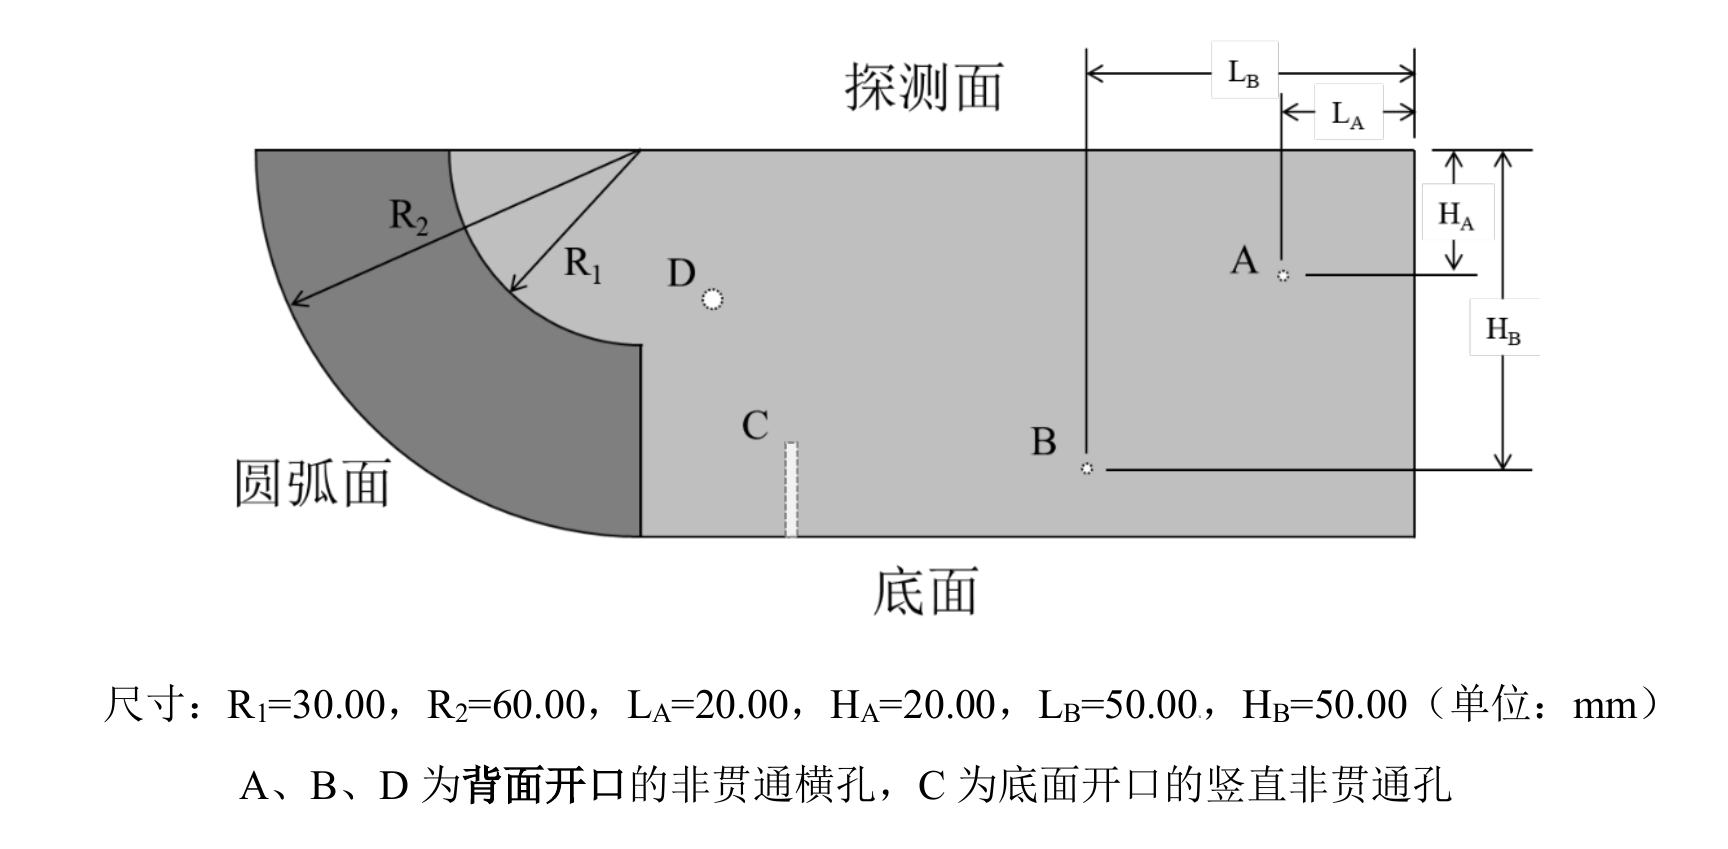
\includegraphics[width=0.85\textwidth]{img/sample.png}
    \caption{测试样尺寸}
    \label{fig:size}
\end{figure}

\textbf{实验数据:}

\begin{table}[!ht]
    \centering
    \caption{声波波速及杨氏模量测量、泊松系数测量}
    \begin{tabular}{|l|l|l|l|}
    \hline
        \textbf{直探头} & \textbf{纵波} & \textbf{斜探头} & \textbf{横波} \\ \hline
        底面回波 & 表面回波 & \(R_2\)弧面回波 & \(R_1\)弧面回波 \\
        峰位(\(t_2/\mu s\)) & 峰位(\(t_1/\mu s\)) & 峰位(\(t_{R_2}/\mu s\)) & 峰位(\(t_{R_1}/\mu s\)) \\ \hline
        19.60 & 0.40 & 48.00 & 28.00 \\ \hline
        19.60 & 0.40 & 49.00 & 29.00 \\ \hline
        19.60 & 0.40 & 49.00 & 29.00 \\ \hline
        \textbf{可变探头} & ── & \textbf{表面波} & ── \\ \hline
        探头角度(\(^{\circ}\)) & 移动距离(\(\Delta_l/mm\)) & 回波峰位(\(t_{S_1}/\mu s\)) & 回波峰位(\(t_{S_2}/\mu s\)) \\ \hline
        68 & 50.0 & 68 & 103 \\ \hline
    \end{tabular}
    \label{table1}
\end{table}

处理数据得到\(\overline{t_2}=19.60\mu s,\overline{t_1}=0.40\mu s\),结合\(l=60.00mm\),计算介质的纵波声速为\[c_l=\df{2\cdot l}{\overline{t_2}-\overline{t_1}}=6.25\times 10^{4}m/s\]

处理数据得到\(\overline{t_{R_2}}=48.67\mu s,\overline{t_{R_1}}=28.67\mu s\),结合\(R_2=60.00mm\),\(R_1=30.00mm\),计算介质的纵波声速为\[c_r=\df{2\cdot(R_2-R_1)}{\overline{t_{R_2}}-\overline{t_{R_1}}}=3.00\times 10^{4}m/s\]

处理数据得到\(\Delta{t_S}=t_{S_2}-t_{S_1}=35\mu s\),结合移动距离\(\Delta l=50.0mm\),计算介质的表面波声速为\[c_s=\df{2\cdot \Delta l}{\Delta{t_S}}=2.86\times 10^{4}m/s\]

则\[T=\df{c_l}{c_r}=2.083\]

则试样的杨氏模量\[E=\df{\rho c_r^2(3T^2-4)}{T^2-1}=65.53GPa\]

试样的 Poisson 系数\[\sigma=\df{T^2-2}{2(T^2-1)}=3.047\times 10^{-1}\]

\subsection{超声波探伤}

\subsubsection{直探头测缺陷深度}

\textbf{实验数据:}

\begin{table}[!ht]
    \centering
    \caption{直探头测缺陷深度}
    \begin{tabular}{|l|l|l|l|l|}
    \hline
        \textbf{直探头(B)} & \textbf{扩散角1} & \textbf{扩散角2} & \textbf{直探头} & \textbf{测缺陷C} \\ \hline
        \(x_0(cm)\) & \(x_1(cm)\) & \(x_2(cm)\) & 底面波(\(t_H-t_1\))(\(\mu s\)) & 缺陷波(\(t_C-t_1\))(\(\mu s\)) \\ \hline
        3.50 & 3.20 & 3.85 & 19.40 & 13.90 \\ \hline
        3.48 & 3.12 & 3.82 & 19.40 & 14.00 \\ \hline
        3.46 & 3.14 & 3.80 & 19.20 & 14.20 \\ \hline
    \end{tabular}
    \label{table2}
\end{table}

计算得到\(\overline{x_2}=3.823cm\),\(\overline{x_1}=3.480cm\),则直探头扩散角为\[\theta=2\arctan\df{\overline{x_2}-\overline{x_1}}{2H_B}=3.933^{\circ}\]

计算得到\(\overline{t_H-t_1}=19.33\mu s\),\(\overline{t_C-t_1}=14.03\mu s\)

计算缺陷深度\[d=H \cdot (1-\df{\overline{t_C-t_1}}{\overline{t_H-t_1}})=16.45mm\]


声速测量计算缺陷深度\[d=c_l \cdot \df{\overline{(t_H-t_1)}-\overline{(t_C-t_1)}}{2}=16.56mm\]

\subsubsection{斜探头测缺陷D}

\textbf{实验数据:}

\begin{table}[!ht]
    \centering
    \caption{斜探头测缺陷D}
    \begin{tabular}{|l|l|l|l|l|l|l|l|l|}
    \hline
        \textbf{斜探头(A)} & \textbf{扩散角1} & \textbf{扩散角2} & \textbf{缺陷A} &  & \textbf{缺陷B} &  & \textbf{缺陷D} &  \\ \hline
        \(x_0(cm)\) & \(x_1(cm)\) & \(x_2(cm)\) & \(x_A(cm)\) & \(t_A(\mu s)\) & \(x_B(cm)\) & \(t_B(\mu s)\) & \(x_D(cm)\) & \(t_D(\mu s)\) \\ \hline
        3.20 & 2.65 & 3.50 & 3.22 & 26.4 & 9.02 & 52.4 & 11.22 & 34.0 \\ \hline
        3.20 & 2.70 & 3.45 & 3.20 & 26.4 & 9.00 & 52.4 & 11.20 & 34.0 \\ \hline
        3.18 & 2.70 & 3.45 & 3.18 & 26.4 & 9.01 & 52.4 & 11.18 & 34.0 \\ \hline
    \end{tabular}
    \label{table3}
\end{table}

计算得到\(\overline{x_A}=3.20cm\),\(\overline{x_B}=9.01cm\),\(\overline{x_D}=11.20cm\),\(\overline{t_A}=26.4\mu s\),\(\overline{t_B}=52.4\mu s\),\(\overline{t_D}=34.0\mu s\),\(\overline{x_2}=3.467cm\),\(\overline{x_1}=2.683cm\)

折射角\[\beta=\arctan\df{(\overline{x_B}-\overline{x_A})-(L_B-L_A)}{H_B-H_A}=43.127^{\circ}\]

则斜探头扩散角为\[\theta=2\arctan(\df{\overline{x_2}-\overline{x_1}}{2\cdot H_A}\cdot\cos\beta)=9.976^{\circ}\]

缺陷D的深度\[H_D=H_B\cdot\df{t_D}{t_B}=32.443mm\]

缺陷D的位置\[L_D=(x_D-H_B\cdot\tan\beta\cdot\df{t_D}{t_B})-(x_B-H_B\cdot\tan\beta)+L_B=88.245mm\]

\newpage
\section{教师签字的原始实验数据}

\begin{figure}[h]
    \centering
    \includegraphics[width=0.85\textwidth]{img/OriginalData.jpg}
    \caption{原始实验数据}
    \label{fig:raw_data_1}
\end{figure}

\end{document}
